\subsection{Experiments with pandoc figures}\label{sec:expt}


\begin{figure}[htbp]
\centering
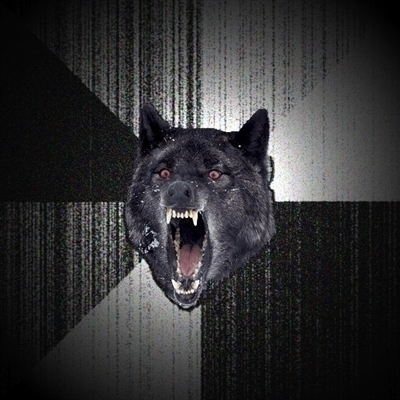
\includegraphics{image.png}
\caption{a figure that can be referred to}
\label{fig:attr}
\end{figure}

Here is a reference to \autoref{fig:attr} and here is one to
\autoref{fig:attr2}.

Here is reference to the section called \autoref{sec:expt}.


\begin{figure}[htbp]
\centering
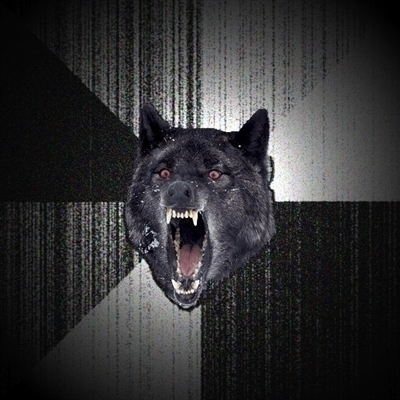
\includegraphics{image.png}
\caption{another figure that can be referred to}
\label{fig:attr2}
\end{figure}

\begin{figure}[htbp]
\centering
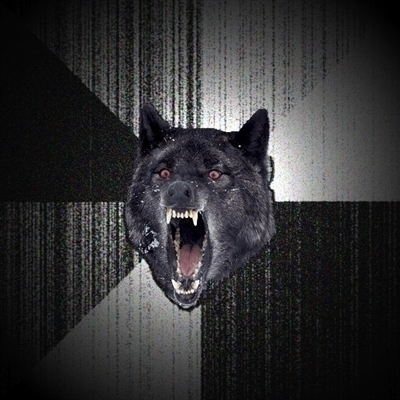
\includegraphics{image.png}
\caption{figure with no attr}
\end{figure}
